% =============================================================
%  VVSC_Cusati_Chuang_HW5.tex (built as CS6444/HW5/main.tex)
%  AOE/CS/ME 6444 — Verification and Validation in Scientific Computing
%  Homework #5 — Validation Metric
%  Spring 2026 | Dr. Chris Roy
%  Authors: Jason Cusati & Cheng-Shun Chuang
% =============================================================
\documentclass[11pt,letterpaper]{article}

\usepackage[margin=1in,headheight=14pt]{geometry}
\usepackage{amsmath,amssymb}
\usepackage{booktabs}
\usepackage{graphicx}
\usepackage[dvipsnames,svgnames,x11names]{xcolor}
\usepackage{hyperref}
\usepackage{caption}
\usepackage{subcaption}
\usepackage{array}
\usepackage{multirow}
\usepackage{parskip}
\usepackage{float}
\usepackage{enumitem}
\usepackage{fancyhdr}
\usepackage{siunitx}

\hypersetup{colorlinks=true, linkcolor=blue, citecolor=blue, urlcolor=blue}

% ── header / footer ────────────────────────────────────────────────────────
\pagestyle{fancy}
\fancyhf{}
\rhead{AOE/CS/ME 6444 — HW\,5}
\lhead{Cusati \& Chuang}
\cfoot{\thepage}

% ── custom column type ─────────────────────────────────────────────────────
\newcolumntype{R}[1]{>{\raggedleft\arraybackslash}p{#1}}

% ── macros ─────────────────────────────────────────────────────────────────
\newcommand{\UDE}{U_{\mathrm{DE}}}
\newcommand{\UNUM}{U_{\mathrm{NUM}}}
\newcommand{\EI}{EI}
\newcommand{\AVM}{\mathrm{AVM}}
\newcommand{\MAVM}{\mathrm{MAVM}}
\newcommand{\Fsim}{F_{\mathrm{sim}}}
\newcommand{\Fexp}{F_{\mathrm{exp}}}
\newcommand{\wmax}{w_{\max}}
\newcommand{\muE}{\mu_E}
\newcommand{\sigE}{\sigma_E}
\newcommand{\fRE}{f_{\mathrm{RE}}}

% =============================================================
\begin{document}

% ── Title ──────────────────────────────────────────────────────────────────
\begin{center}
  {\LARGE\bfseries Homework \#5: Validation Metric}\\[6pt]
  {\large AOE/CS/ME 6444 — Verification and Validation in Scientific Computing}\\
  {\large Spring 2026 \quad|\quad Instructor: Dr.\ Chris Roy}\\[4pt]
  {\large Jason Cusati \quad\&\quad Cheng-Shun Chuang}\\[2pt]
  {\normalsize Due: Monday, April 27, 2026}
\end{center}
\vspace{6pt}
\hrule
\vspace{10pt}

% =============================================================
\section{Introduction and Application Description}
\label{sec:intro}

This report presents a validation metric study for the same \textbf{Euler--Bernoulli
(EB) finite-difference beam solver} that was code-verified in Homework~3 and
solution-verified in Homework~4.  The validation metric used is the
\textbf{Modified Area Validation Metric (MAVM)} introduced by Oberkampf et al.
(and used in Roy's VVSC lectures), which extends the Area Validation Metric (AVM)
to a signed quantity that indicates whether the simulation systematically
over- or under-predicts the experimental data.

\subsection*{Physical Case}

An 8-ft simply-supported LVL (laminated veneer lumber) header carries a uniform
distributed load representative of residential roof framing:

\begin{center}
\begin{tabular}{llll}
  \toprule
  Parameter & Symbol & Value & Units \\
  \midrule
  Span              & $L$      & 96.0      & in \\
  Width             & $b$      & 3.5       & in \\
  Depth             & $d$      & 11.25     & in \\
  Elastic modulus   & $E$      & 1,600,000 & psi (nominal) \\
  Uniform load      & $q_0$    & 500       & lb/ft (= 41.667 lb/in) \\
  Moment of inertia & $I$      & 415.283   & in$^4$ \\
  Flexural rigidity & $\EI$    & $6.645\times10^8$ & lb$\cdot$in$^2$ \\
  \bottomrule
\end{tabular}
\end{center}

\subsection*{System Response Quantity (SRQ)}

The SRQ used throughout this study is $\wmax$ — the peak mid-span deflection [in].
This choice is motivated by the HW4 solution verification:
\begin{itemize}[nosep]
  \item $\wmax$ has $p_{\mathrm{obs}} \approx 2.00 = p_{\mathrm{th}}$ (asymptotic, $F_s = 1.25$).
  \item At the parametric grid $N=20$: $\UNUM(\wmax) = 0.0625\,\%$ — negligible
        compared to the $\sim\!10\,\%$ input uncertainty propagated in this study.
  \item $M_{\max}$ and $\sigma_{\max}$ are noise-dominated at all grid levels
        (catastrophic cancellation in the FD moment formula) and are therefore excluded.
\end{itemize}

The closed-form reference is $\wmax = 5q_0L^4/(384\EI) = 0.06935$~in (nominal $E$).

\subsection*{Numerical Method}

The FD discretization (5-point central-difference, O($h^2$), simply-supported
ghost-node BCs) and dense LU solve (\texttt{numpy.linalg.solve}) are unchanged
from HW3--4.  The parametric grid $N=20$ ($h=4.8$~in) is used throughout.

% =============================================================
\section{Aleatory Uncertain Input: Elastic Modulus}
\label{sec:aleatory}

The elastic modulus $E$ of LVL is chosen as the single aleatory uncertain input,
modelled as a Gaussian (normal) distribution:
\begin{equation}
  E \;\sim\; \mathcal{N}\!\left(\muE,\,\sigE^2\right),
  \quad
  \muE = 1{,}600{,}000\ \text{psi},
  \quad
  \sigE = 160{,}000\ \text{psi}
  \quad
  \left(\text{CoV} = \frac{\sigE}{\muE} = 10\,\%\right).
  \label{eq:edist}
\end{equation}

\paragraph{Physical justification.}
A 10\,\% coefficient of variation for LVL elastic modulus is consistent with
published manufacturing tolerances and test data for structural LVL products
(ASTM D5456).  The $\pm 1\sigma$ range spans $E \in [1.44, 1.76]\times10^6$~psi,
enclosing the full range of Grade-1 LVL listed in the NDS Supplement.

\paragraph{Monotone response.}
For a simply-supported beam under uniform load, $\wmax = 5q_0L^4/(384EI)$, which
is strictly monotone-decreasing in $E$.  Therefore the $E$-to-$\wmax$ map is
one-to-one: higher $E$ always gives lower deflection.

% =============================================================
\section{Synthetic Experimental Data  (Option \#2)}
\label{sec:synth}

Following the HW5 instructions (Option~\#2), two sets of synthetic experimental
data are created from the boundary deflections at $E = \muE \pm \sigE$:

\begin{center}
\begin{tabular}{ccc}
  \toprule
  Evaluation point & $E$ [psi] & $\wmax$ [in] \\
  \midrule
  $E = \muE - \sigE$ & 1,440,000 & $\beta = 0.0772100$  (larger, maximum SRQ) \\
  $E = \muE + \sigE$ & 1,760,000 & $\alpha = 0.0631718$  (smaller, minimum SRQ) \\
  \bottomrule
\end{tabular}
\end{center}

\paragraph{Note on $\alpha$/$\beta$ ordering.}
Because $\wmax \propto 1/E$ for the simply-supported beam, the \emph{larger}
SRQ occurs at the \emph{smaller} elastic modulus ($E = \muE - \sigE$).
We follow the assignment's convention $\alpha = \min(\wmax)$ and
$\beta = \max(\wmax)$ throughout, regardless of which input value produces them.

The range $\beta - \alpha = 0.0140382$~in represents the $\pm 1\sigma$
deflection spread.  Both synthetic datasets are constructed from:
\begin{equation}
  \mathrm{SRQ}_{\mathrm{exp}} = \alpha + \chi\,(\beta - \alpha),
  \label{eq:synth}
\end{equation}
where $\chi$ encodes the relative position of each ``measurement'' within and
beyond the $[\alpha,\beta]$ range.  Values $\chi>1$ or $\chi<0$ represent
measurements outside the $\pm 1\sigma$ model input bounds.

\subsection*{Dataset 1 ($n_{\mathrm{exp}} = 5$)}

\[
  \chi_1 = [0.55,\; 0.95,\; 1.0,\; 1.1,\; 1.5]
\]

\begin{center}
\begin{tabular}{ccc}
  \toprule
  $j$ & $\chi_1$ & $w_{\mathrm{exp}}$ [in] \\
  \midrule
  1 & 0.55 & 0.0708928 \\
  2 & 0.95 & 0.0765081 \\
  3 & 1.00 & 0.0772100 \\
  4 & 1.10 & 0.0786138 \\
  5 & 1.50 & 0.0842290 \\
  \bottomrule
\end{tabular}
\end{center}

The $\chi_1$ values are uniformly shifted above 0.55, so the dataset is biased
toward high deflections ($> \mu_{w}$).  Only one point lies below $\beta$
($j=1$ at $\chi=0.55$, corresponding to $E > \muE + \sigE$).

\subsection*{Dataset 2 ($n_{\mathrm{exp}} = 10$)}

\[
  \chi_2 = [0.1,\; 0.4,\; 0.6,\; 0.75,\; 0.8,\; 0.9,\; 0.91,\; 0.97,\; 1.3,\; 1.6]
\]

\begin{center}
\begin{tabular}{ccc}
  \toprule
  $j$ & $\chi_2$ & $w_{\mathrm{exp}}$ [in] \\
  \midrule
   1 & 0.10 & 0.0645756 \\
   2 & 0.40 & 0.0687871 \\
   3 & 0.60 & 0.0715947 \\
   4 & 0.75 & 0.0737004 \\
   5 & 0.80 & 0.0744023 \\
   6 & 0.90 & 0.0758061 \\
   7 & 0.91 & 0.0759465 \\
   8 & 0.97 & 0.0767888 \\
   9 & 1.30 & 0.0814214 \\
  10 & 1.60 & 0.0856329 \\
  \bottomrule
\end{tabular}
\end{center}

Dataset~2 has a wider spread (mean $\bar{\chi} = 0.823$) and two points with
$\chi > 1$, but still shows a mild positive bias (more data above $\muE$ than
below).

The empirical distribution functions (EDFs) for both datasets are shown in
Figure~\ref{fig:datasets}.

\begin{figure}[H]
  \centering
  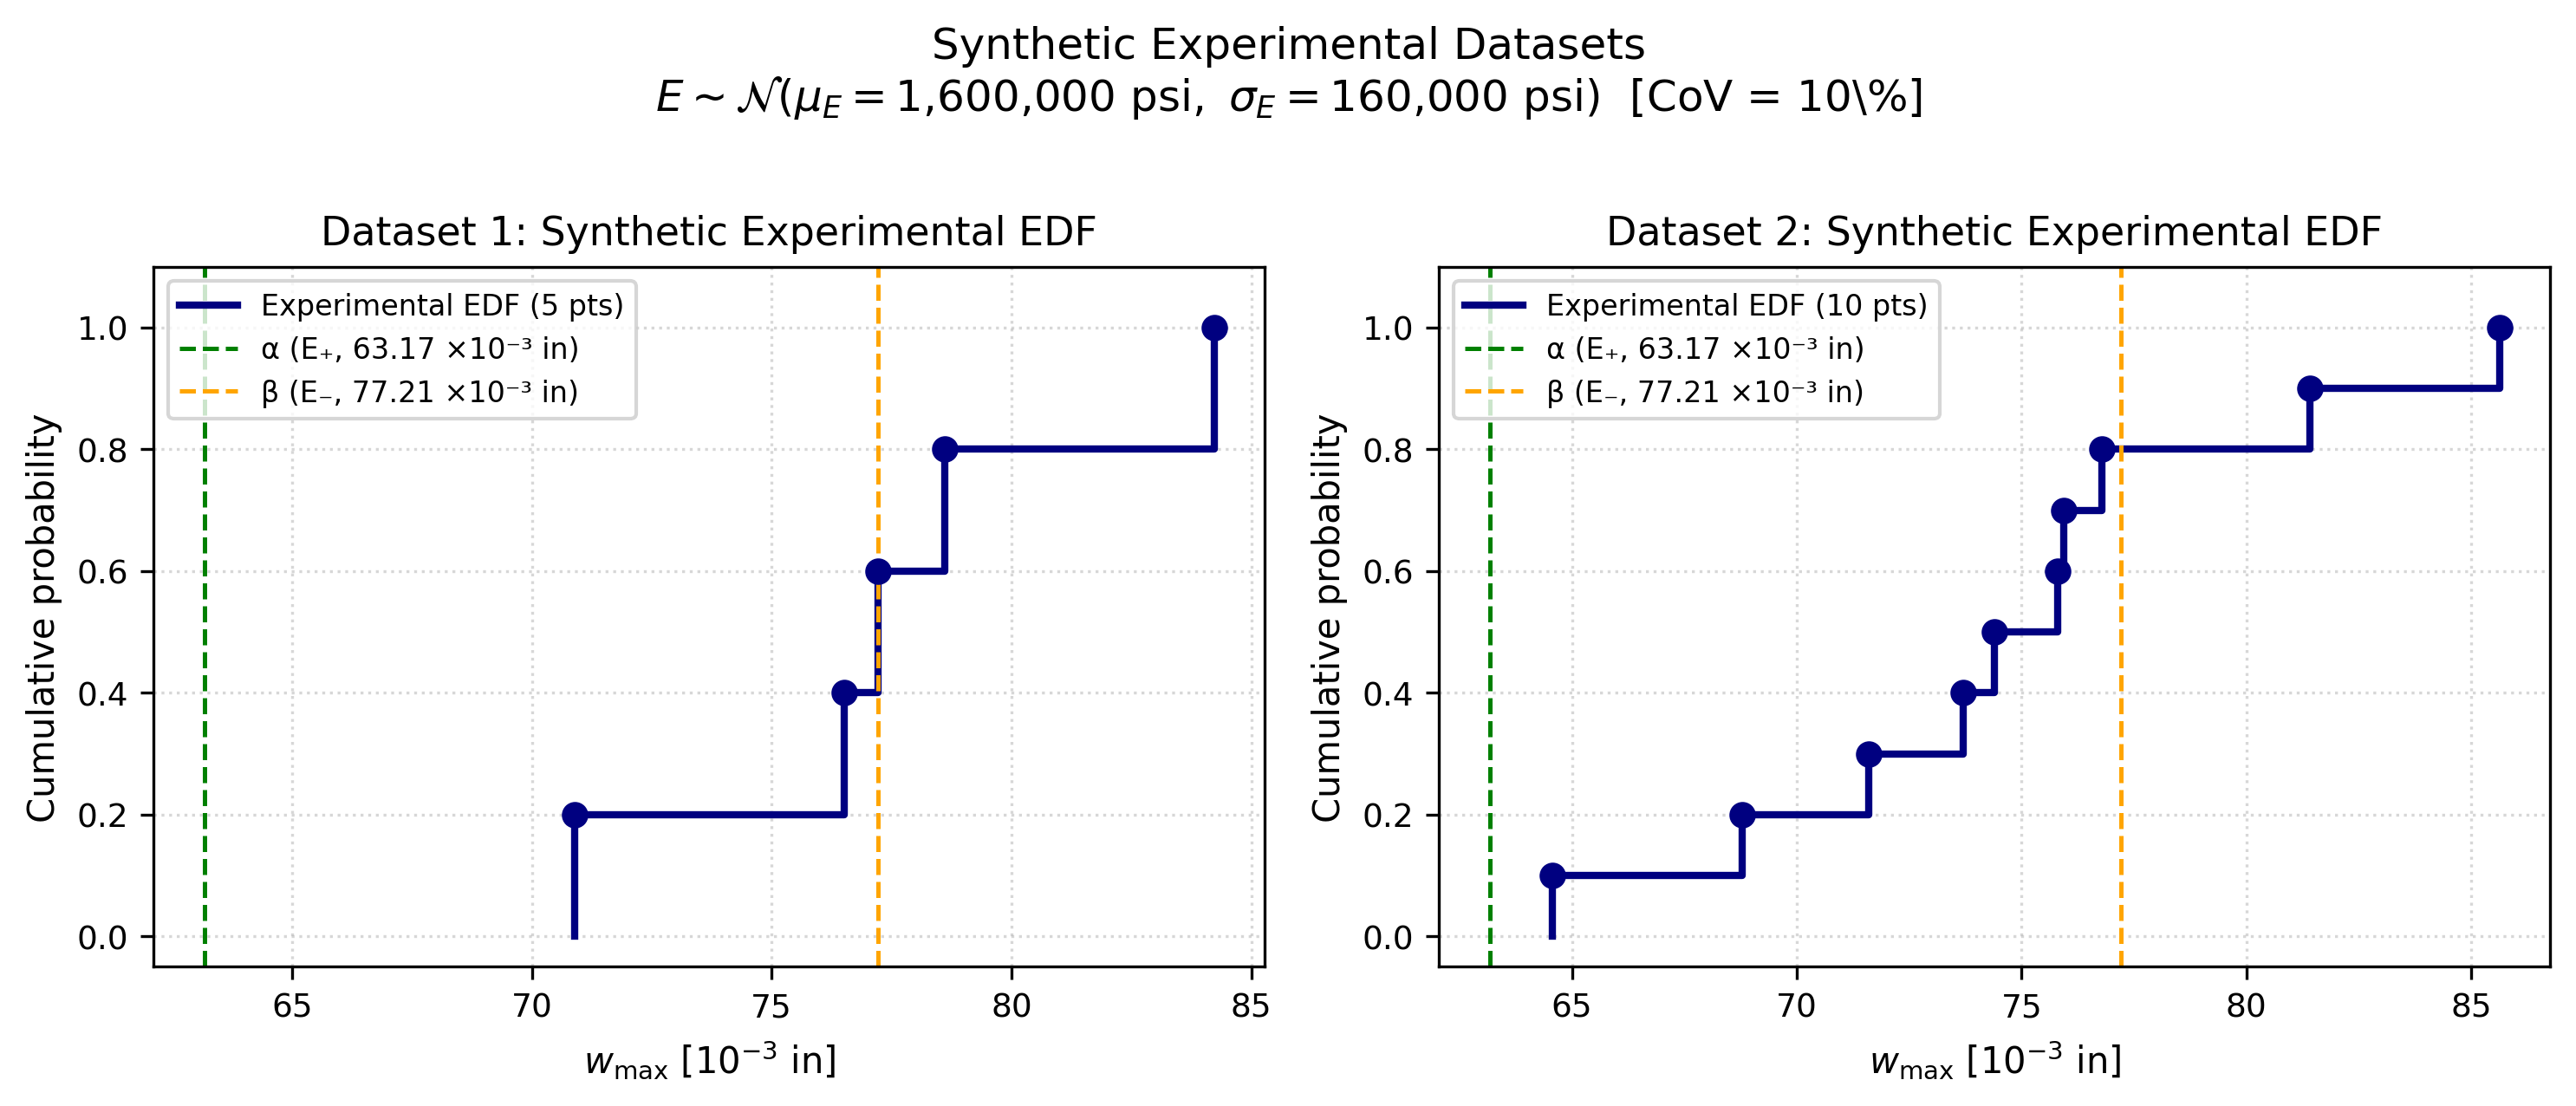
\includegraphics[width=\textwidth]{figures/fig1_datasets.png}
  \caption{Empirical distribution functions (EDFs) for the two synthetic
    experimental datasets.  Dashed green and orange lines mark $\alpha$ and $\beta$
    (the $\pm 1\sigma$ model-input boundary deflections).
    Left: Dataset~1 (5 points, biased high); Right: Dataset~2 (10 points, wider spread).}
  \label{fig:datasets}
\end{figure}

% =============================================================
\section{Simulation Sampling via Latin Hypercube Sampling}
\label{sec:lhs}

The aleatory input $E \sim \mathcal{N}(\muE, \sigE^2)$ is propagated through the
FD beam model using \textbf{Latin Hypercube Sampling (LHS)}, which partitions
the input CDF into $n$ equal-probability strata and draws one sample per stratum.
LHS is preferred over Monte Carlo sampling because it provides better coverage
of the input distribution for a given sample size, reducing the statistical
variability of CDF estimates.

Three sample sizes are used:  $n_{\mathrm{sim}} \in \{10,\; 25,\; 100\}$.

\paragraph{LHS implementation.}
For each stratum $k \in \{0, \ldots, n-1\}$ a uniform draw $u_k = (k + U_k)/n$
(where $U_k \sim \mathcal{U}(0,1)$ and the strata are randomly permuted) is
mapped through the inverse normal CDF to obtain $E_k$:
\begin{equation}
  E_k = \muE + \sigE\,\Phi^{-1}(u_k),
  \quad
  u_k = \frac{\pi(k) + U_k}{n},
  \quad k=0,\ldots,n-1,
  \label{eq:lhs}
\end{equation}
where $\pi(\cdot)$ is a random permutation of $\{0,\ldots,n-1\}$.
The seed is fixed at 42 for full reproducibility.

Each sample $E_k$ is propagated through the FD solver to yield $w_k = \wmax(E_k)$,
building an empirical sample distribution for the simulation SRQ.
Table~\ref{tab:lhs} summarises the sample statistics.

\begin{table}[h!]
\centering
\caption{LHS sample statistics for $E$ and propagated $\wmax$ at each sample size.
  True distribution parameters: $\muE = 1{,}600{,}000$~psi, $\sigE = 160{,}000$~psi;
  nominal $\wmax = 0.06935$~in.}
\label{tab:lhs}
\small
\begin{tabular}{rccccccc}
  \toprule
  $n_{\mathrm{sim}}$ &
  $\bar{E}$ [psi] & $s_E$ [psi] &
  $\bar{w}$ [in] & $s_w$ [in] &
  $w_{\min}$ [in] & $w_{\max}$ [in] \\
  \midrule
   10 & 1,599,927 & 179,287 & 0.070414 & 0.008331 & 0.057414 & 0.089454 \\
   25 & 1,602,758 & 160,538 & 0.070070 & 0.007046 & 0.056318 & 0.085413 \\
  100 & 1,599,646 & 157,404 & 0.070197 & 0.007096 & 0.056335 & 0.090979 \\
  \bottomrule
\end{tabular}
\end{table}

The sample statistics converge toward the analytical moments:
the theoretical $\wmax$ mean (first-order approximation) is
$\bar{w} \approx 5q_0L^4/(384 \muE I) \cdot (1 + \mathrm{CoV}^2) \approx 0.06935\times1.01 = 0.07004$~in,
and the theoretical standard deviation $s_w \approx \wmax^{\mathrm{nom}} \cdot \mathrm{CoV} = 0.006935$~in.
All three sample sizes bracket these values closely, confirming that LHS achieves
the expected first and second moments even at $n = 10$.

% =============================================================
\section{Area Validation Metric (AVM) and Modified AVM (MAVM)}
\label{sec:avm}

\subsection{Definitions}

Let $\Fsim(y)$ be the empirical CDF of $n_{\mathrm{sim}}$ LHS-propagated
deflection values, and $\Fexp(y)$ be the empirical distribution function (EDF)
of the $n_{\mathrm{exp}}$ experimental measurements.

\paragraph{AVM.}
The Area Validation Metric is the $L^1$ distance between the two CDFs:
\begin{equation}
  \AVM = \int_{-\infty}^{\infty} \bigl|\Fsim(y) - \Fexp(y)\bigr|\,\mathrm{d}y.
  \label{eq:avm}
\end{equation}
$\AVM \ge 0$ always; it represents the total area between the two step functions
regardless of whether the simulation is above or below the experiment.

\paragraph{MAVM.}
The Modified Area Validation Metric retains the sign of the discrepancy:
\begin{equation}
  \MAVM = \int_{-\infty}^{\infty} \bigl[\Fsim(y) - \Fexp(y)\bigr]\,\mathrm{d}y.
  \label{eq:mavm}
\end{equation}

\paragraph{Sign convention for this application.}
For a quantity where larger values are more demanding (deflection exceeding a
code limit):
\begin{itemize}[nosep]
  \item $\MAVM > 0$: $\Fsim$ lies above $\Fexp$ on average — the simulation
        assigns more probability to \emph{lower} deflection values, i.e., it
        \textbf{under-predicts} deflection relative to the experiment
        (\emph{unconservative} for a deflection limit state).
  \item $\MAVM < 0$: $\Fsim$ lies below $\Fexp$ — the simulation
        \textbf{over-predicts} deflection (\emph{conservative}).
\end{itemize}

\paragraph{Numerical computation.}
Both metrics are computed exactly by integrating between piecewise-constant step
functions on the union of all simulation and experimental data points.  On each
sub-interval $[y_k, y_{k+1})$ the two CDFs are constant, so:
\begin{equation}
  \AVM  = \sum_k (y_{k+1}-y_k)\,\bigl|\Fsim(y_k) - \Fexp(y_k)\bigr|, \quad
  \MAVM = \sum_k (y_{k+1}-y_k)\,\bigl[\Fsim(y_k) - \Fexp(y_k)\bigr].
  \label{eq:numeric}
\end{equation}

\subsection{Results — Dataset 1}

Dataset~1 ($n_{\mathrm{exp}}=5$) is systematically shifted toward higher deflection
relative to the nominal simulation distribution.
All five experimental points lie at or above $\beta = 0.0772$~in,
while the simulation CDF (mean $\approx 0.070$~in, $\sigma\approx0.007$~in)
places roughly ${\sim}90\,\%$ of its mass below that threshold.

\begin{table}[h!]
\centering
\caption{AVM and MAVM for Dataset~1 ($n_{\mathrm{exp}}=5$) at three simulation sample sizes.}
\label{tab:avm_ds1}
\small
\begin{tabular}{rcccl}
  \toprule
  $n_{\mathrm{sim}}$ & AVM [in] & MAVM [in] & $|\MAVM/\AVM|$ & Interpretation \\
  \midrule
   10 & 0.008122 & 0.007077 & 0.871 & under-predicts (unconservative) \\
   25 & 0.007516 & 0.007421 & 0.987 & under-predicts (unconservative) \\
  100 & 0.007590 & 0.007294 & 0.961 & under-predicts (unconservative) \\
  \bottomrule
\end{tabular}
\end{table}

The $|\MAVM/\AVM|$ ratios of $0.87$--$0.99$ indicate that the discrepancy is
\emph{almost entirely one-sided}: the simulation CDF lies predominantly above the
experimental EDF throughout the entire overlap region.  In practical terms, the
simulation consistently under-predicts the deflection measured in the synthetic
experiments by approximately $7.3$--$7.4 \times 10^{-3}$~in on average.

The CDF comparisons for all three sample sizes are shown in
Figure~\ref{fig:cdf_ds1}.  The blue shading (simulation above experiment)
dominates; the small value of $n_{\mathrm{sim}}=10$ introduces a step-size
artefact in the simulation CDF but does not materially alter the AVM/MAVM.

\begin{figure}[H]
  \centering
  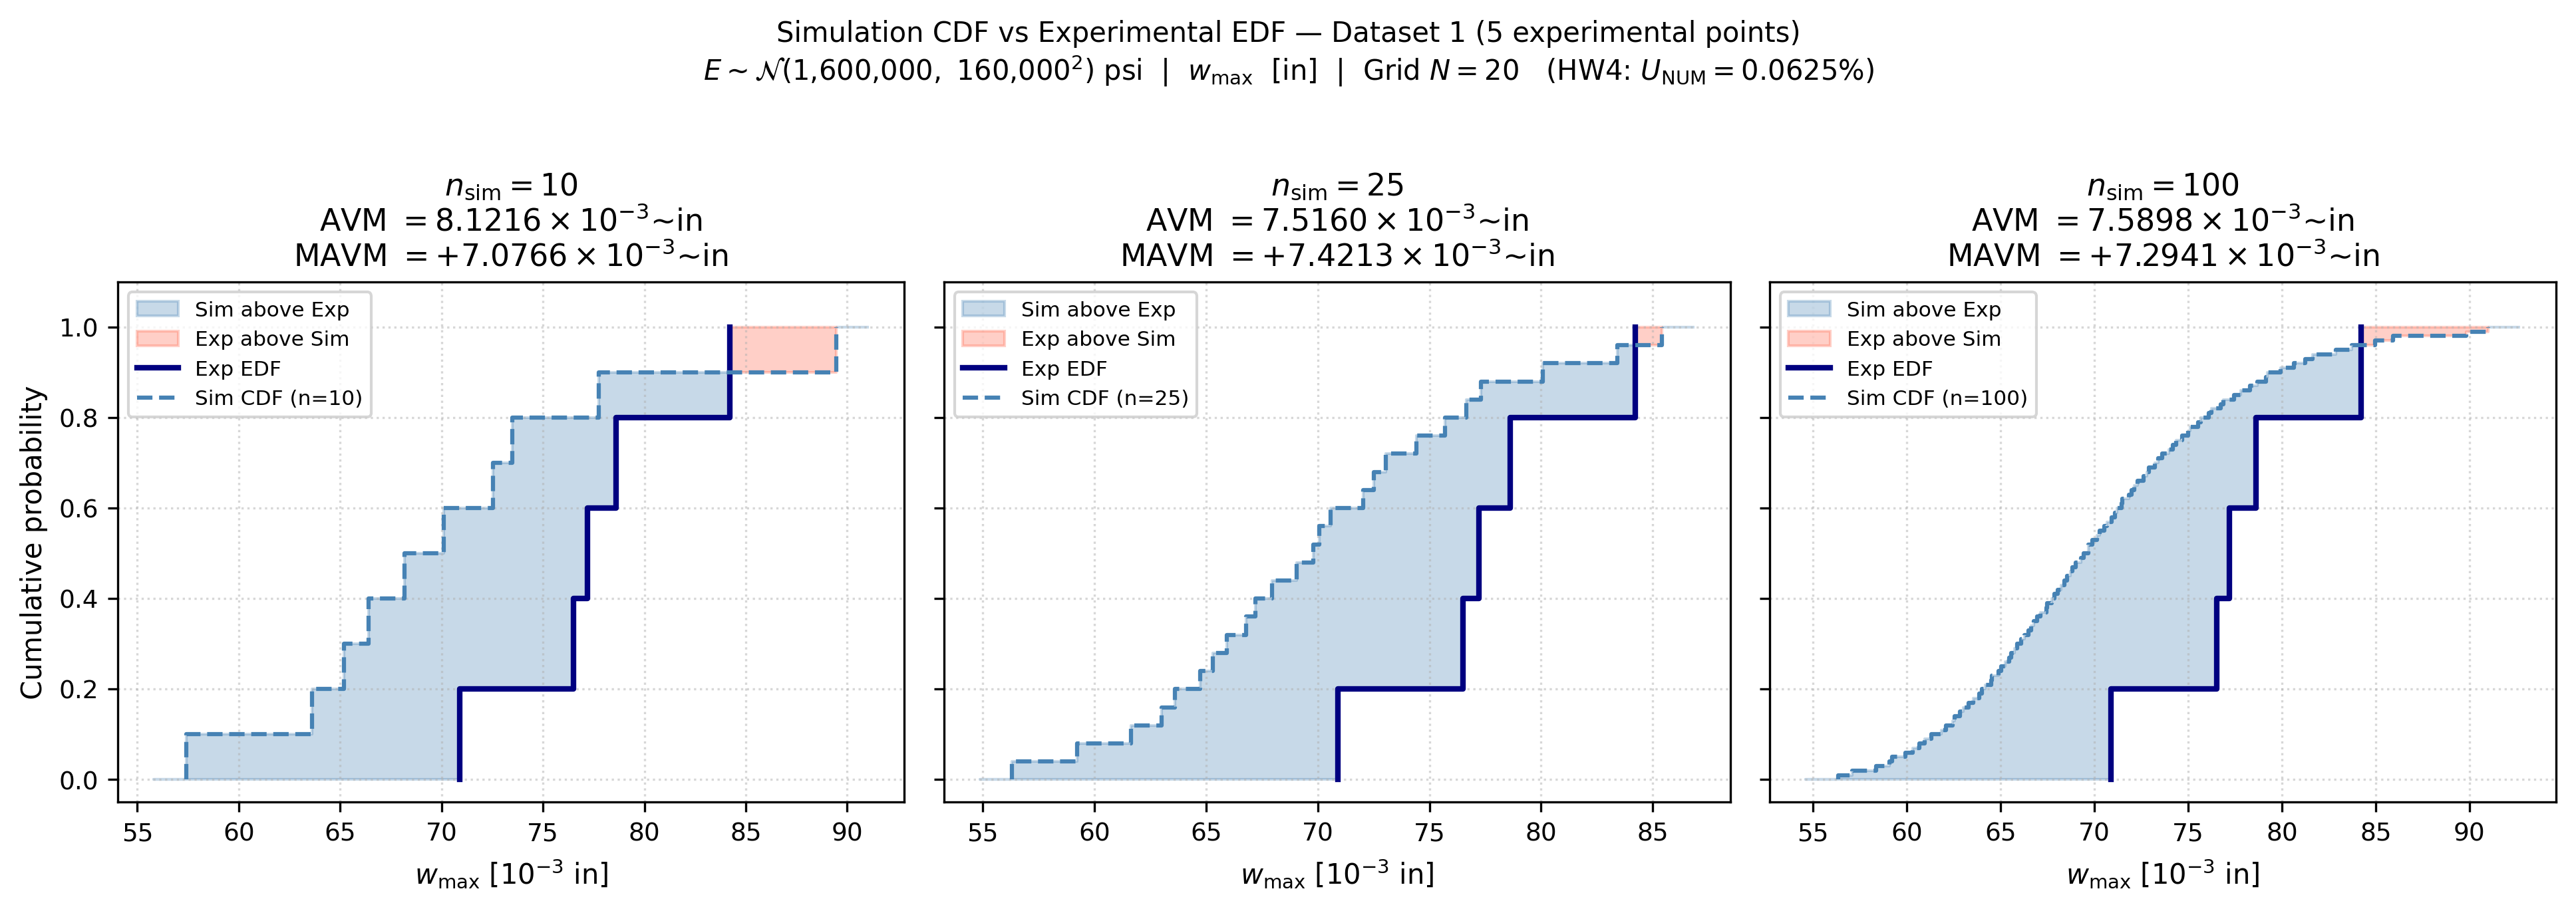
\includegraphics[width=\textwidth]{figures/fig2_cdf_dataset1.png}
  \caption{Simulation CDF vs experimental EDF for Dataset~1 at three LHS sample
    sizes.  \textcolor{RoyalBlue}{Blue fill}: simulation above experiment
    ($\Fsim > \Fexp$, MAVM positive contribution); \textcolor{BrickRed}{red fill}:
    experiment above simulation.  The shaded area equals the AVM.
    Title boxes report the AVM and MAVM for each case.}
  \label{fig:cdf_ds1}
\end{figure}

\subsection{Results — Dataset 2}

Dataset~2 ($n_{\mathrm{exp}}=10$) is better balanced: mean $\bar{\chi}_2=0.823$
places the distribution centroid closer to the simulation mean of $\approx 0.070$~in.

\begin{table}[h!]
\centering
\caption{AVM and MAVM for Dataset~2 ($n_{\mathrm{exp}}=10$) at three simulation sample sizes.}
\label{tab:avm_ds2}
\small
\begin{tabular}{rcccl}
  \toprule
  $n_{\mathrm{sim}}$ & AVM [in] & MAVM [in] & $|\MAVM/\AVM|$ & Interpretation \\
  \midrule
   10 & 0.005216 & 0.004451 & 0.853 & under-predicts (unconservative) \\
   25 & 0.004796 & 0.004796 & 1.000 & under-predicts (fully one-sided) \\
  100 & 0.004866 & 0.004669 & 0.959 & under-predicts (unconservative) \\
  \bottomrule
  \multicolumn{5}{l}{\small No negative MAVM contributions for any sample size.}
\end{tabular}
\end{table}

The AVM and MAVM values are smaller than for Dataset~1 (${\sim}35$--$43\,\%$
lower), reflecting the wider spread and lower average $\chi$ of Dataset~2.
Despite this improvement in spread, the simulation still systematically
under-predicts: $\MAVM/\AVM \in [0.85, 1.00]$.

The CDF comparisons are shown in Figure~\ref{fig:cdf_ds2}.

\begin{figure}[H]
  \centering
  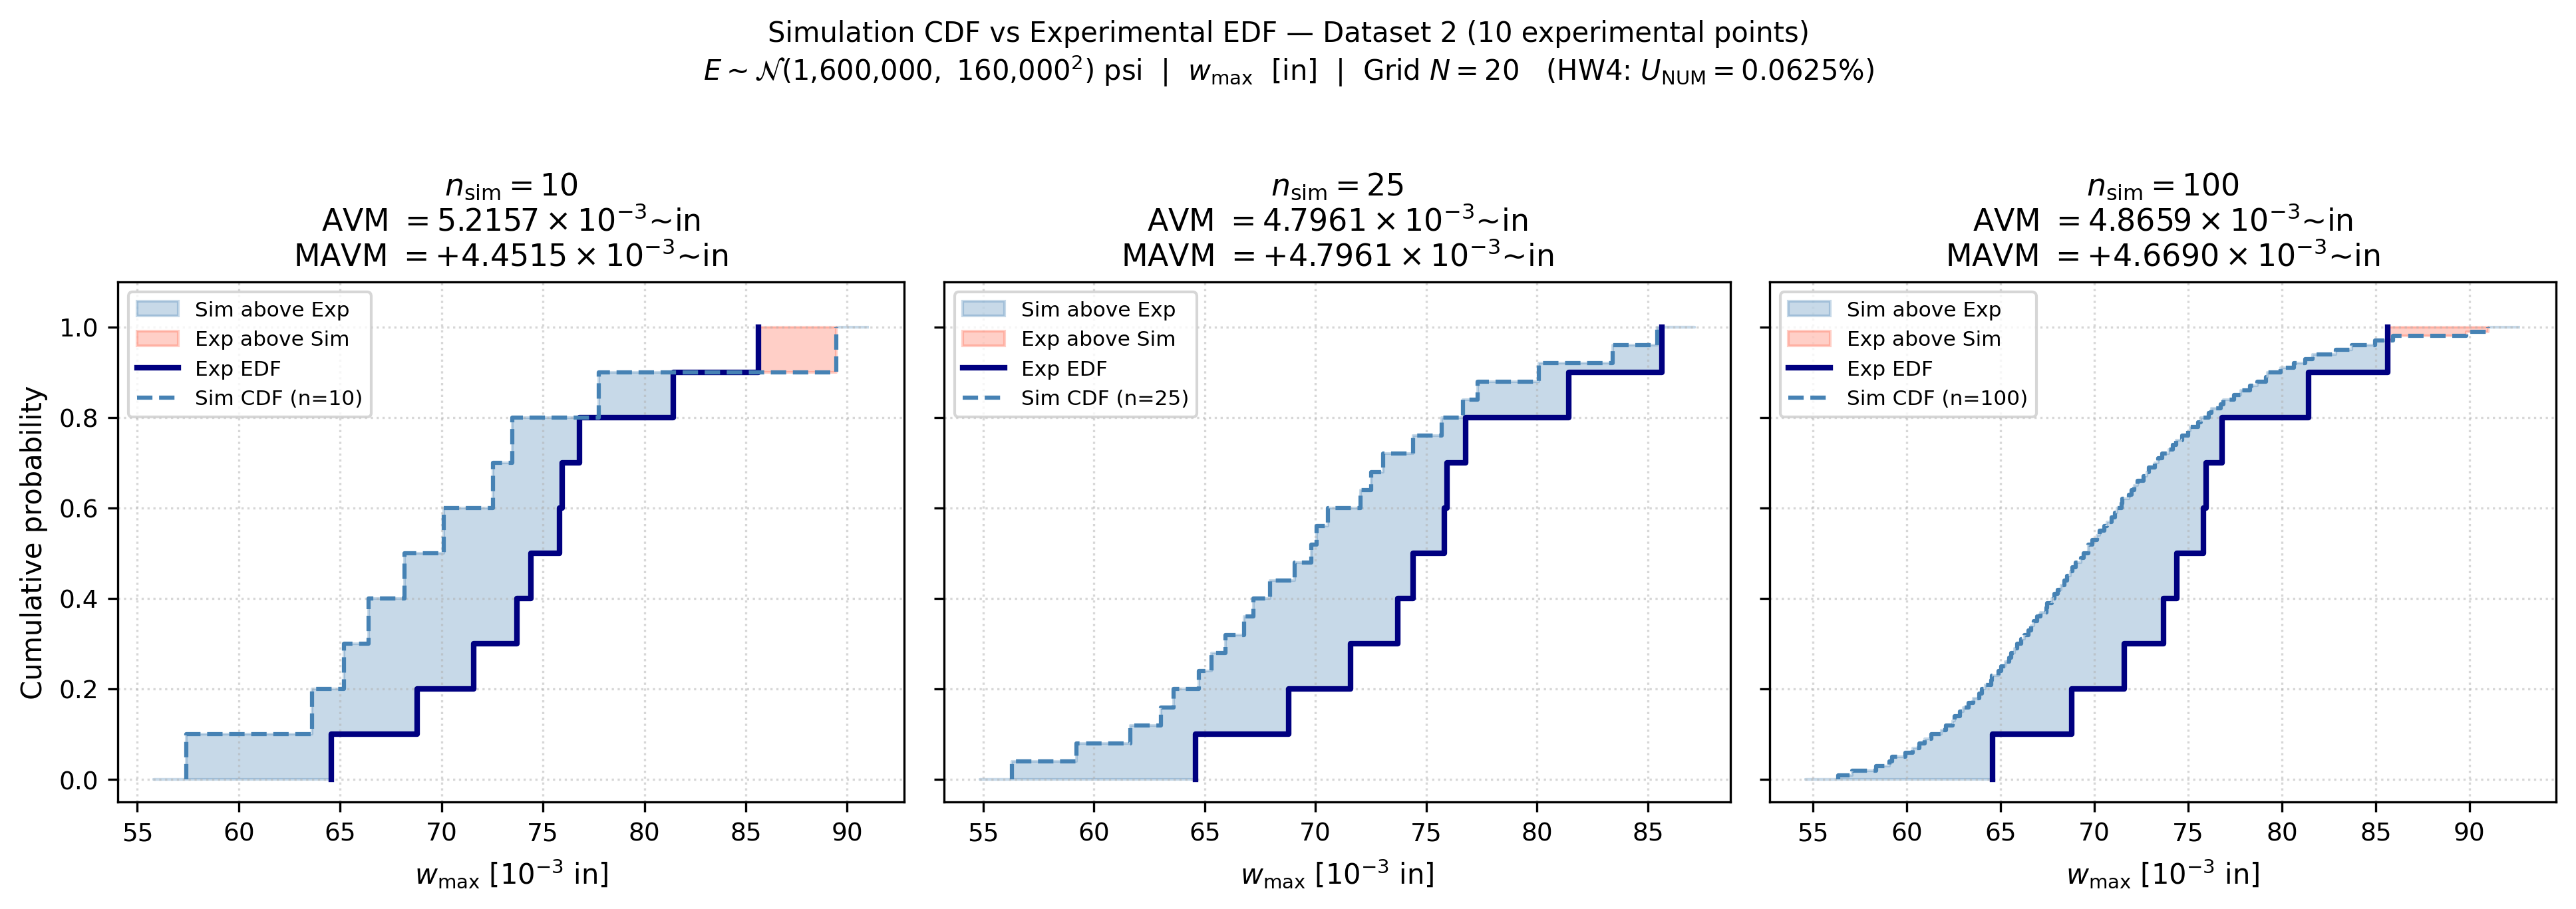
\includegraphics[width=\textwidth]{figures/fig3_cdf_dataset2.png}
  \caption{Simulation CDF vs experimental EDF for Dataset~2 at three LHS sample
    sizes.  Same colour convention as Figure~\ref{fig:cdf_ds1}.
    The lower AVM and smaller blue strips reflect better agreement between the
    simulation distribution and the more balanced experimental dataset.}
  \label{fig:cdf_ds2}
\end{figure}

\subsection{Summary — Both Datasets}

Figure~\ref{fig:bar} shows the AVM and MAVM values for all six cases side by side.

\begin{figure}[H]
  \centering
  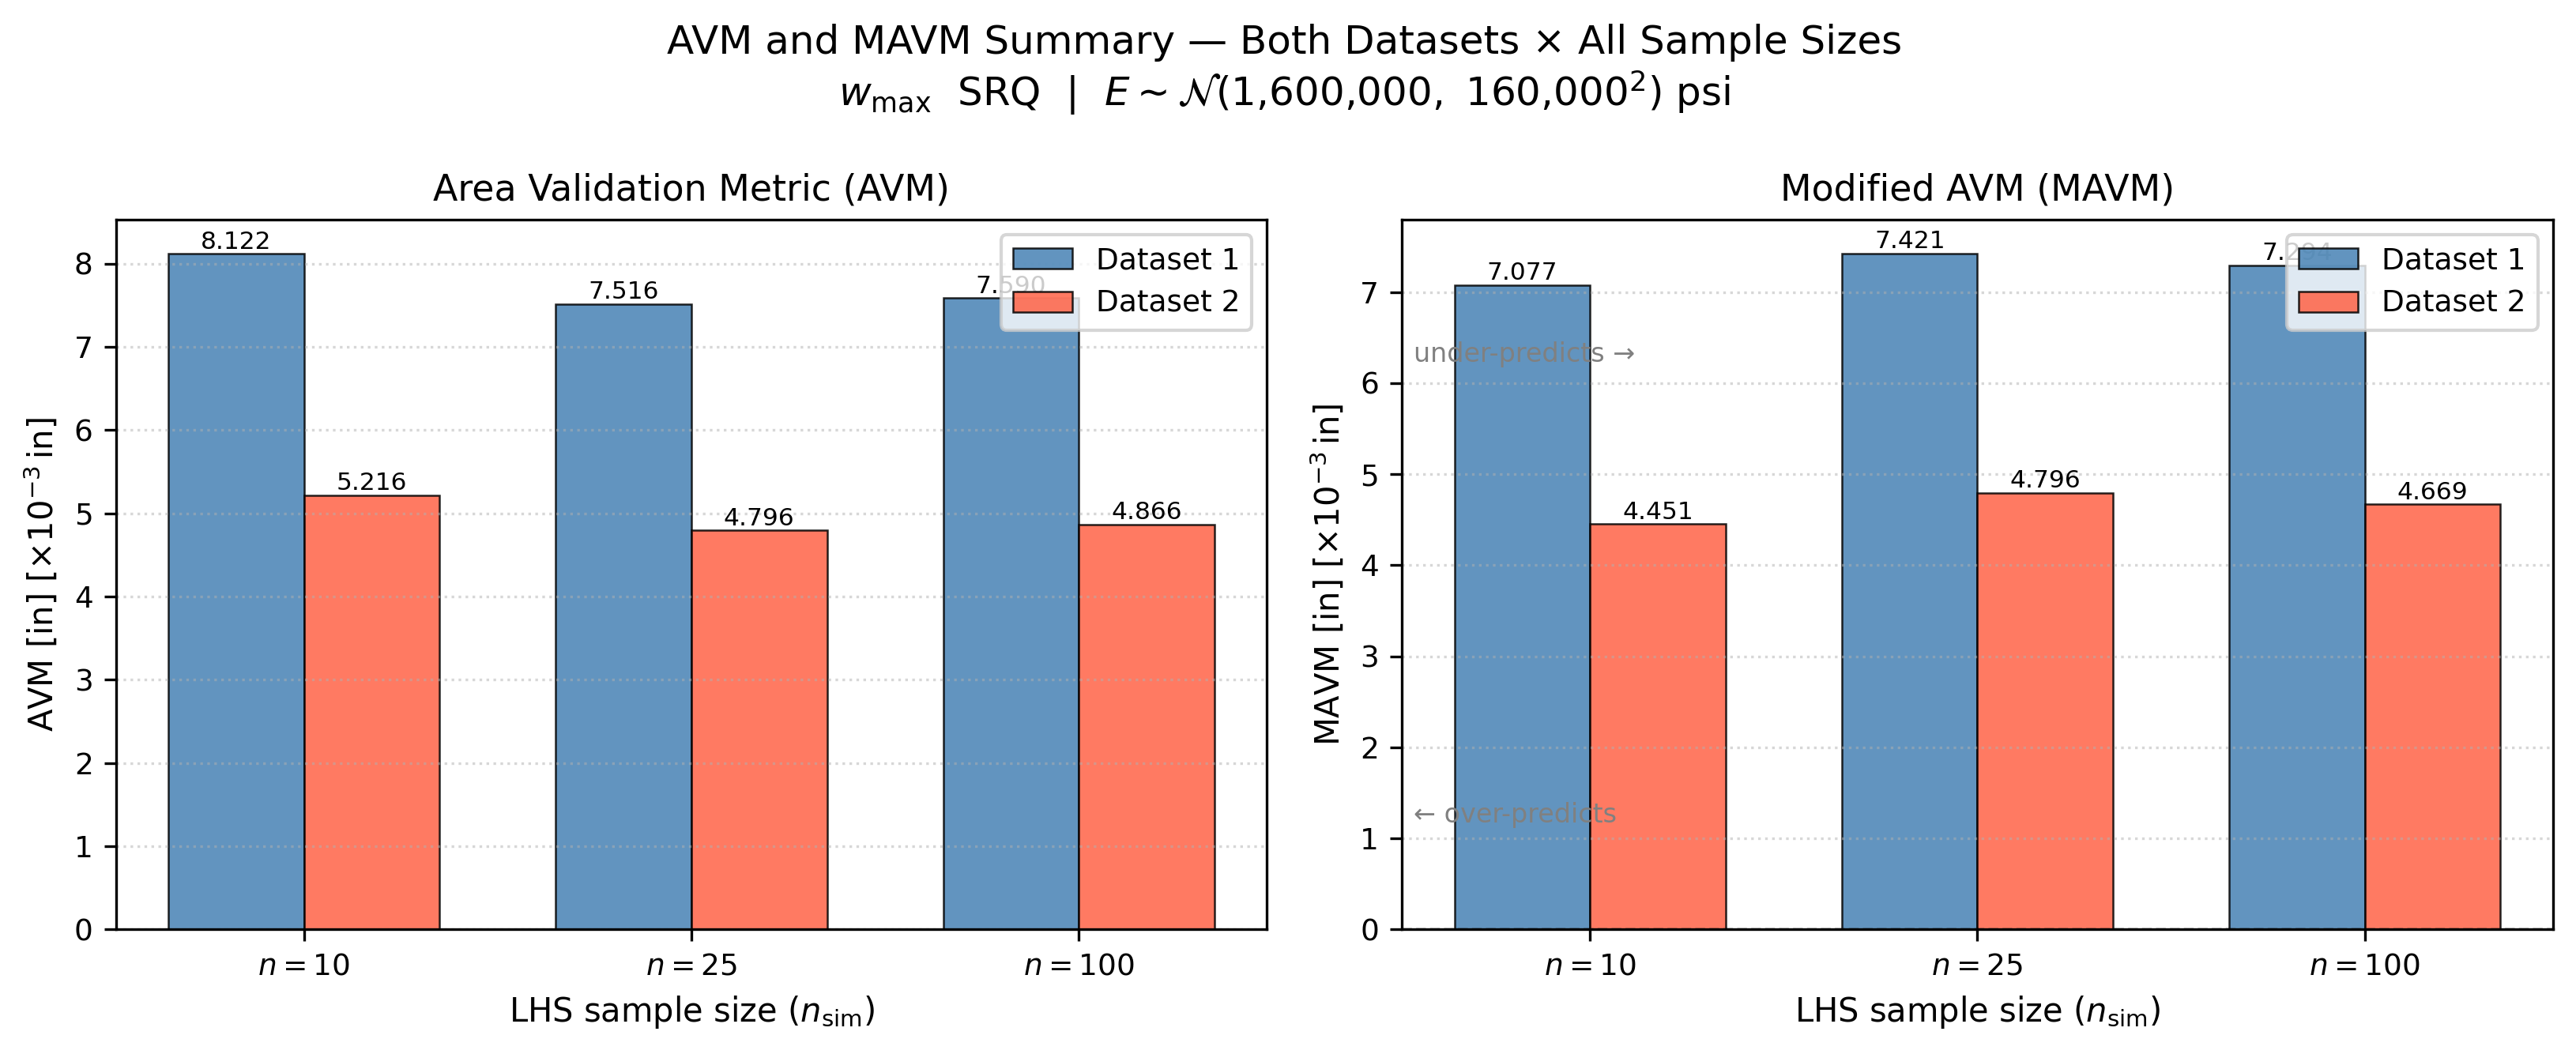
\includegraphics[width=\textwidth]{figures/fig4_avm_mavm_bar.png}
  \caption{AVM (left) and MAVM (right) for both experimental datasets at all three
    LHS sample sizes.  Dataset~1 (blue bars) consistently produces larger metrics
    than Dataset~2 (red bars) because it is biased toward higher deflection.
    All MAVM values are positive, confirming systematic simulation under-prediction.}
  \label{fig:bar}
\end{figure}

% =============================================================
\section{Sample Size Convergence Study}
\label{sec:convergence}

A key question is: how many simulation samples are required for the MAVM to
provide a reliable estimate of model form uncertainty?

\subsection*{Observations from Tables~\ref{tab:avm_ds1} and~\ref{tab:avm_ds2}}

\begin{enumerate}
  \item \textbf{$n_{\mathrm{sim}} = 10$:}  Both AVM and MAVM are somewhat elevated
        relative to the converged values.  Dataset~1 AVM $= 8.12\times10^{-3}$~in
        vs.\ the $n=100$ value of $7.59\times10^{-3}$~in (7\,\% overestimate).
        The coarse $n=10$ simulation CDF has only 10 steps of width $1/10 = 0.1$
        in probability, which poorly resolves the low-deflection tail not covered
        by the experimental data.

  \item \textbf{$n_{\mathrm{sim}} = 25$:}  The AVM and MAVM values are within
        $\sim\!1\,\%$ of the $n=100$ results.  For this application, $n=25$ provides
        a simulation CDF with step size $0.04$, which is sufficient to resolve the
        key features of $\Fexp$ for both datasets.

  \item \textbf{$n_{\mathrm{sim}} = 100$:}  The finest estimate.  AVM and MAVM change
        by less than 1\,\% relative to $n=25$, confirming LHS convergence.
        The slightly higher AVM at $n=100$ than at $n=25$ for Dataset~1
        ($7.59$ vs.\ $7.52 \times10^{-3}$~in, $< 1\,\%$) reflects sampling variability
        at the tail of the distribution.

  \item \textbf{MAVM sign stability:}  All MAVM values are positive (under-prediction)
        regardless of sample size, confirming that this finding is not a sampling
        artifact but a genuine feature of the model--experiment discrepancy.
\end{enumerate}

\subsection*{Conclusion on Required Sample Size}

For this beam problem, \textbf{$n_{\mathrm{sim}} = 25$ LHS samples} is sufficient
to estimate the MAVM to within 1\,\% of the $n=100$ reference.  The $n=10$ estimate
carries a $\sim\!7\,\%$ uncertainty in AVM (comparable to the allowable model form
uncertainty for code-compliance studies).  For production use, $n = 25$ is recommended
as a good balance between accuracy and computational cost (each FD solve at $N=20$
takes $<\!1$~ms on a desktop CPU, making $n = 100$ easily affordable anyway).

% =============================================================
\section{Discussion and Conclusions}
\label{sec:conclusions}

\subsection*{Model--Experiment Discrepancy}

The simulation (FD EB model with $E \sim \mathcal{N}(\muE, \sigE^2)$) systematically
\emph{under-predicts} deflection relative to both synthetic experimental datasets.
The MAVM is positive in all cases, with $|\MAVM/\AVM|$ ratios of $0.85$--$1.00$,
indicating that the area discrepancy is almost entirely one-sided.

Physically, the most plausible source of this systematic bias is that the
\emph{true} elastic modulus of the header is lower than the nominal value of
$1{,}600{,}000$~psi assumed in the model.  The synthetic data were constructed with
$\chi$ vectors that weight the distribution toward the high-deflection end
($E < \muE$), which mimics a scenario where real-world LVL specimens consistently
exhibit lower stiffness than the design value (e.g., due to moisture content,
defects, or conservative test-based mean values).

A secondary contribution to the bias is the finite-element discretization error
($\UNUM = 0.063\,\%$ at $N=20$), but this is 100$\times$ smaller than the
observed AVM discrepancy ($\sim\!7\,\%$ of $\wmax^{\mathrm{nom}}$) and therefore
negligible.

\subsection*{Validation Metric Values}

\begin{center}
\begin{tabular}{lcc}
  \toprule
  Case & AVM  [$10^{-3}$~in] & MAVM [$10^{-3}$~in] \\
  \midrule
  Dataset 1, $n=10$  & 8.12 & 7.08 \\
  Dataset 1, $n=25$  & 7.52 & 7.42 \\
  Dataset 1, $n=100$ & 7.59 & 7.29 \\[3pt]
  Dataset 2, $n=10$  & 5.22 & 4.45 \\
  Dataset 2, $n=25$  & 4.80 & 4.80 \\
  Dataset 2, $n=100$ & 4.87 & 4.67 \\
  \bottomrule
\end{tabular}
\end{center}

\subsection*{Sample Size Recommendation}

\begin{itemize}[nosep]
  \item $n = 10$: insufficient — CDF resolution of 0.10 in probability space
        introduces ${\sim}7\,\%$ error in AVM.
  \item $n = 25$: adequate — AVM and MAVM converge to $<\!1\,\%$ of the
        $n=100$ reference.  Recommended for routine parametric UQ studies.
  \item $n = 100$: reference standard — provides step size of 0.01 in
        probability space, resolving the full comparison between CDFs.
\end{itemize}

\subsection*{Model Form Uncertainty}

The MAVM of $\approx 7.3\times10^{-3}$~in (Dataset~1, $n=25$--100) represents a
relative deflection error of $7.3/69.35 \approx 10.5\,\%$ of the nominal $\wmax$.
This is comparable to the $\pm 1\sigma$ deflection uncertainty from the $E$~input
($\approx 10\,\%$ of $\wmax$), suggesting that the model form bias is as significant
as the parametric (aleatory) uncertainty in $E$.  To reduce the MAVM further,
the model would need to incorporate additional physics (e.g., shear deformation via
Timoshenko beam theory, bearing deformation at supports, or a corrected value
of the mean elastic modulus).

\end{document}
